\pagebreak
\section{Steering test - Linear Area for \si{K_p}} \label{app:LinearAreaKp}
\textbf{Name: Group 510}\\
\textbf{Date: 30/09 - 2015}

\subsubsection{Purpose}
The purpose of this test is to find a minimum and maximum value of the \si{K_P} for the steering controller.

\subsubsection{Setup}


\subsubsection{List of Equipment}

\begin{table}[H]
\begin{tabular}{|p{10cm}|p{4cm}|}
\hline%------------------------------------------------------------------------------------
  \textbf{Instrument}                     &  \textbf{Type}       \\
\hline%------------------------------------------------------------------------------------
  Computer                                &  Acer C720p    \\
\hline %-----------------------------------------------------------------------------------
\end{tabular}
\end{table}

\subsubsection{Procedure}

\begin{enumerate}
  \item Disconnect the battery.
  \item Connect the Arduino to the computer.
  \item Upload the test code to the Arduino board using the Arduino IDE  \cite{ArduinoIDE}.
  \item Plug in the battery
  \item Open a serial terminal via PuTTY \cite{PuTTY} immediately after plugging the battery.
  \item Wait two seconds, then follow the vehicle with the connected computer.
  \item Wait until the vehicle stops before ending the measurements by unplugging the connected computer from the Arduino.
  \item Plot the angle of the vehicle using Matlab.
\end{enumerate}

\subsubsection{Results}

By utilizing 20 measurements, where three is illustrated in \figref{steeringPlotSpeedVsGain}, 20 time-constants is found by using the formula from \eqref{SteeringTimeconstant}.

\begin{figure}[H]
  \centering
 	%Trim margins @:   left        bottom       right       top
 	\adjustbox{ trim = {.15\width} {.30\height} {.15\width} {.30\height}, clip }
  {
    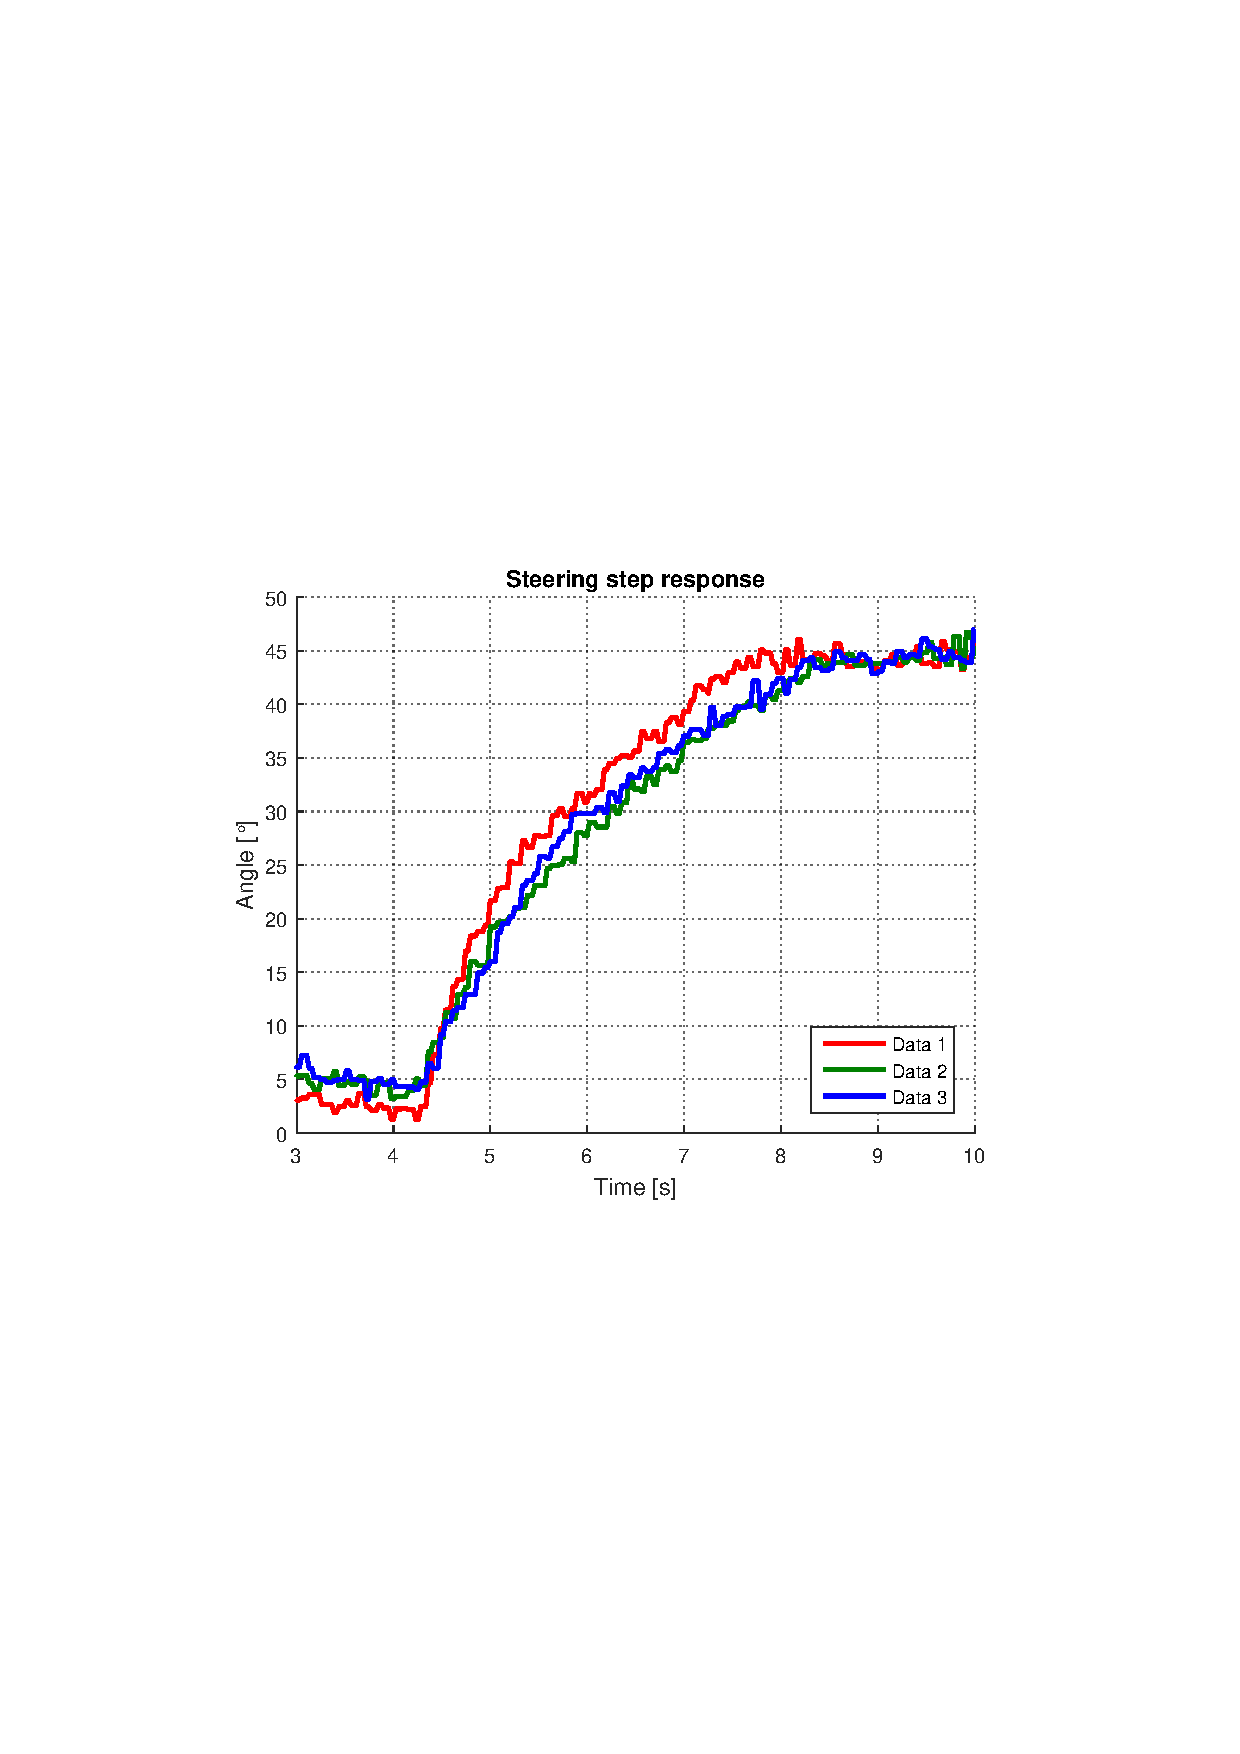
\includegraphics[width=1.4\textwidth]{figures/steeringStep_P2.pdf}
  }
  \caption{Plot of three test where the vehicle is turning, where the x-axis is time and the y-axis is angle.}
  \label{steeringPlotSpeedVsGain}
\end{figure}
%
\begin{table}[H]
\begin{tabular}{|p{2cm}|p{2cm}|p{3cm}|p{2cm}|p{2cm}|p{3cm}|}
\hline%-----------------------------------------------------------------------------------------------------------------
\textbf{Test}  &  \textbf{\si{\tau}} &  \textbf{\si{\tau}}  &  \textbf{Test}   &  \textbf{\si{\tau}}  &    \textbf{\si{\tau}}        \\
\hline%-----------------------------------------------------------------------------------------------------------------
           1    &  1  &   0.180831826   &   10    &     2.5    &           0.344827586              \\
\hline%-----------------------------------------------------------------------------------------------------------------
           2    &   1   &   0.180342651   &  11    &      2.5    &        0.294117647                 \\
\hline%-----------------------------------------------------------------------------------------------------------------
           3    &   1  &    0.17088175   &  12    &       2.5     &           0.291970803              \\
\hline%-----------------------------------------------------------------------------------------------------------------
           4    &  1.5  &   0.266666667   &   13   &       3     &         0.362318841                \\
\hline%-----------------------------------------------------------------------------------------------------------------
           5    &  1.5  &   0.259403372   &   14   &        3    &         0.256410256                \\
\hline%-----------------------------------------------------------------------------------------------------------------
           6    &  1.5  &   0.254452926   &    15    &       3.5     &          0.840336134               \\
\hline%-----------------------------------------------------------------------------------------------------------------
           7    &  2  &  0.265957447    &   16    &          3.5     &            0.549450549             \\
\hline%-----------------------------------------------------------------------------------------------------------------
           8    & 2  &   0.284090909   &    17   &            3.5     &           0.476190476              \\
\hline%-----------------------------------------------------------------------------------------------------------------
           9    & 2  &   0.37037037    &    18    &           4       &         0.549450549                \\
\hline%-----------------------------------------------------------------------------------------------------------------
\end{tabular}
\end{table}

og beregner kv ud fra data og plotter

\begin{figure}[H]
  \centering
 	%Trim margins @:   left        bottom       right       top
 	\adjustbox{ trim = {.15\width} {.30\height} {.15\width} {.30\height}, clip }
  {
    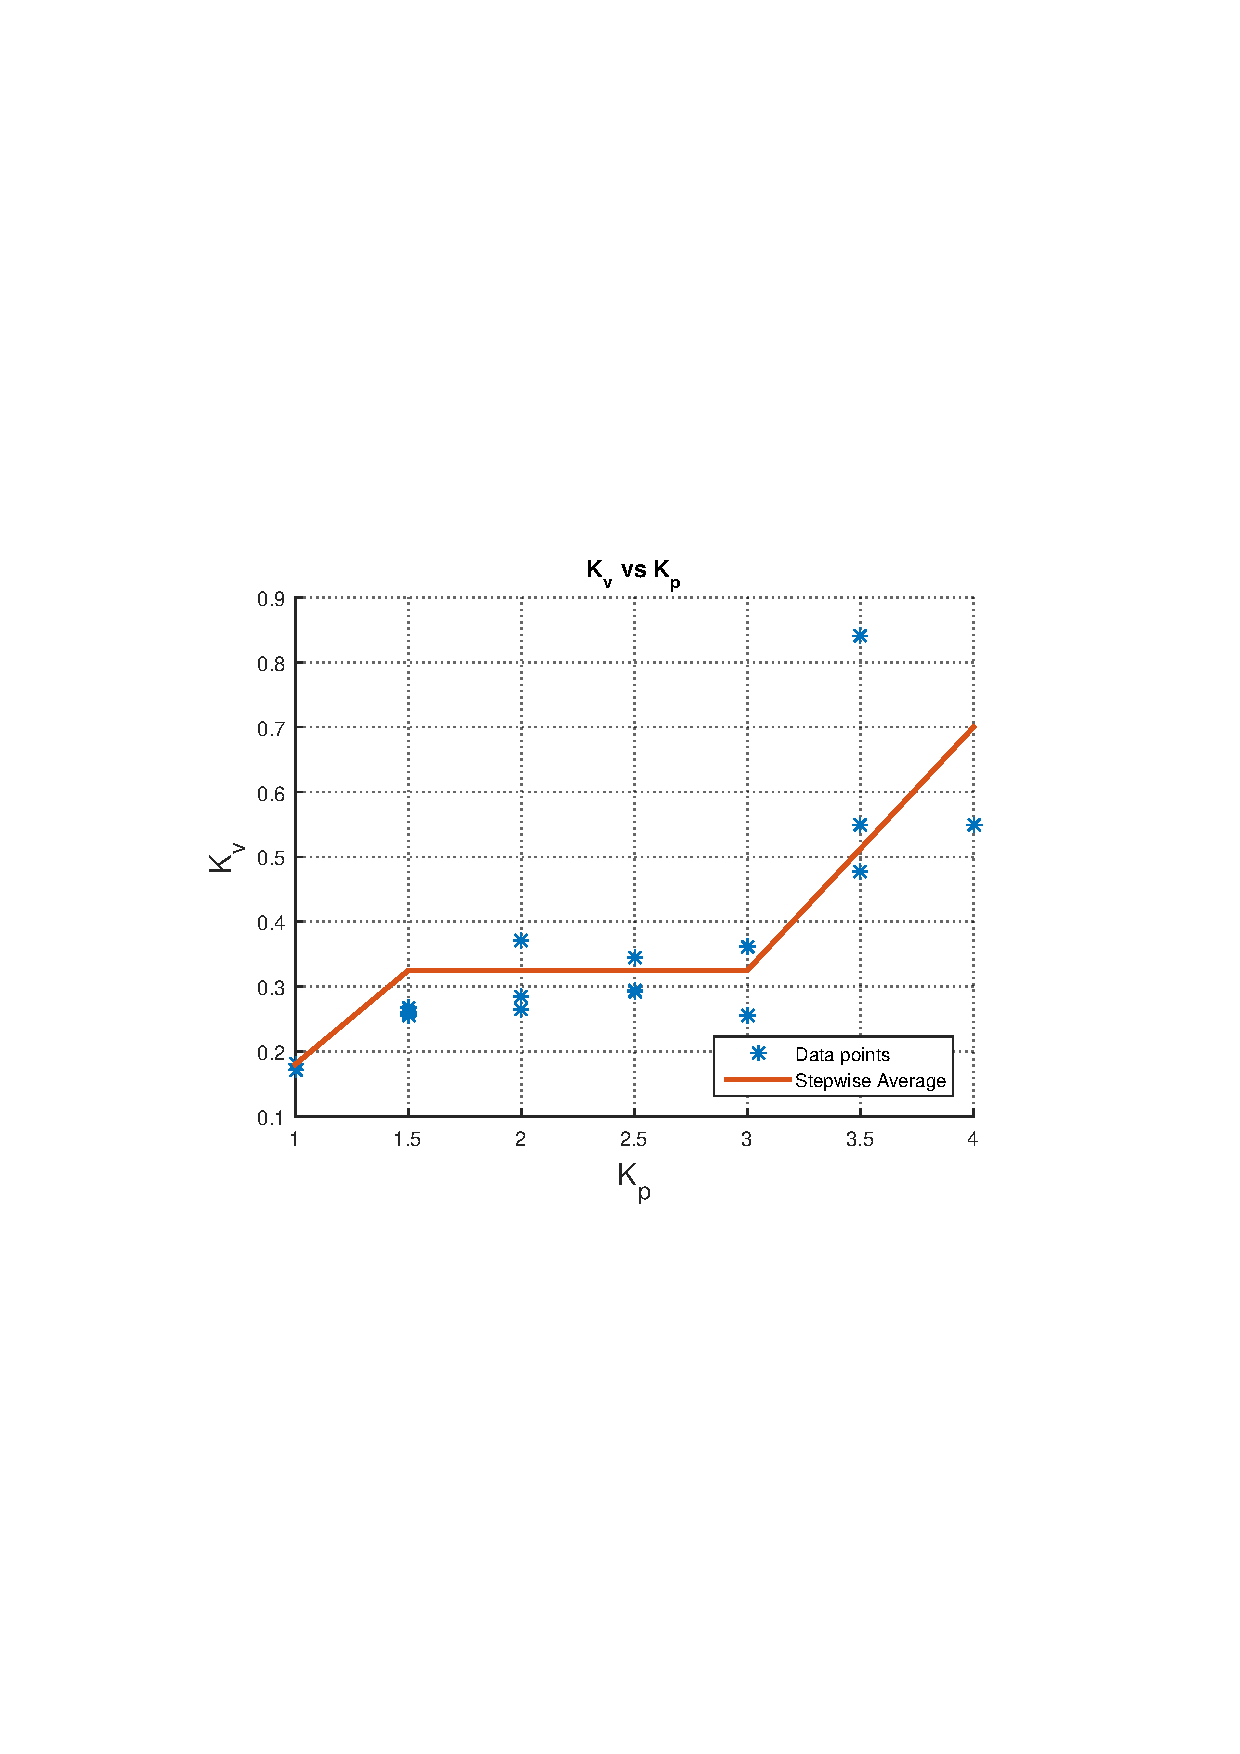
\includegraphics[width=1.4\textwidth]{figures/KvKpSteeringtest.pdf}
  }
  \caption{Plot of the gain \si{K_v} against the real speed.}
  \label{steeringPlotSpeedVsGain}
\end{figure}
%
